\documentclass[letterpaper]{article}
\usepackage[margin=1in]{geometry}
\usepackage[utf8]{inputenc}
\usepackage{textcomp}
\usepackage{amssymb}
\usepackage{natbib}
\usepackage{graphicx}
\usepackage{gensymb}
\usepackage{amsthm, amsmath, mathtools}
\usepackage[dvipsnames]{xcolor}
\usepackage{enumerate}
\usepackage{mdframed}
\usepackage[most]{tcolorbox}
\usepackage{csquotes}
% https://tex.stackexchange.com/questions/13506/how-to-continue-the-framed-text-box-on-multiple-pages

\tcbuselibrary{theorems}

\newcommand{\R}{\mathbb{R}}
\newcommand{\Z}{\mathbb{Z}}
\newcommand{\N}{\mathbb{N}}
\newcommand{\Q}{\mathbb{Q}}
\newcommand{\C}{\mathbb{C}}
\newcommand{\code}[1]{\texttt{#1}}
\newcommand{\mdiamond}{$\diamondsuit$}
\newcommand{\PowerSet}{\mathcal{P}}
\newcommand{\Mod}[1]{\ (\mathrm{mod}\ #1)}
\DeclareMathOperator{\lcm}{lcm}

%\newtheorem*{theorem}{Theorem}
%\newtheorem*{definition}{Definition}
%\newtheorem*{corollary}{Corollary}
%\newtheorem*{lemma}{Lemma}
\newtheorem*{proposition}{Proposition}


\newtcbtheorem[number within=section]{theorem}{Theorem}
{colback=green!5,colframe=green!35!black,fonttitle=\bfseries}{th}

\newtcbtheorem[number within=section]{definition}{Definition}
{colback=blue!5,colframe=blue!35!black,fonttitle=\bfseries}{def}

\newtcbtheorem[number within=section]{corollary}{Corollary}
{colback=yellow!5,colframe=yellow!35!black,fonttitle=\bfseries}{cor}

\newtcbtheorem[number within=section]{lemma}{Lemma}
{colback=red!5,colframe=red!35!black,fonttitle=\bfseries}{lem}

\newtcbtheorem[number within=section]{example}{Example}
{colback=white!5,colframe=white!35!black,fonttitle=\bfseries}{def}

\newtcbtheorem[number within=section]{note}{Important Note}{
        enhanced,
        sharp corners,
        attach boxed title to top left={
            xshift=-1mm,
            yshift=-5mm,
            yshifttext=-1mm
        },
        top=1.5em,
        colback=white,
        colframe=black,
        fonttitle=\bfseries,
        boxed title style={
            sharp corners,
            size=small,
            colback=red!75!black,
            colframe=red!75!black,
        } 
    }{impnote}
\usepackage[utf8]{inputenc}
\usepackage[english]{babel}
\usepackage{fancyhdr}
\usepackage[hidelinks]{hyperref}

\pagestyle{fancy}
\fancyhf{}
\rhead{MATH 155A}
\chead{Tuesday, April 05, 2022}
\lhead{Lecture 3}
\rfoot{\thepage}

\setlength{\parindent}{0pt}

\begin{document}

\section{Introduction to Shader Programs}
\subsection{Sending Data from a C++ Program to a Shader Program}
There are three ways to send data to a shader program. 
\begin{enumerate}
    \item \textbf{Per-Vertex Vertex Attribute:} Here, a vertex attribute is a data value associated with a particular vertex. These are stored in the VBO, and generally different values for each vertex. 
    \item \textbf{Generic Vertex Attribute:} These are the same values for all vertices in a single draw command (e.g. \code{glDrawArrays} or \code{glDrawElements}). These can change between calls, though. 
    \item \textbf{Uniform Variables:} Essentially the same as generic vertex attributes. 
\end{enumerate}
Note that the values in (1) and (2), vertex attributes, can be accessed only by the vertex shader. However, uniform values, like (3), can be accessed by both the vertex and fragment shader.

\subsubsection{Per-Vertex Attributes}
We make use of the \code{glBindBuffer} and \code{glBufferData} commands to load vertex attributes into a VBO. We also use \code{glVertexAttribPointer} to tell the VAO the information about what vertex attributes are in the VBO, and where they are. We can also use \code{glEnableVertexAttribArray} to enable the data from the VBO. 

\subsubsection{Generic Attributes}
We use \code{glDisableVertexAttribArray} and \code{glVertexAttrib3f}\footnote{\code{3f} means three floats.} to set a generic attribute's value. 

\subsubsection{Uniform Variables}
For matrices, we use \code{glUniformMatrixfv} to set the values in a $4 \times 4$ matrix in column order. We use \code{GetUniformLocation} to get the ``location number'' of the uniform variable.





\newpage 
\section{Graphics Pipeline, Linear \& Affine Transformations in \texorpdfstring{$\R^2$}{R2}}
The graphics pipelines, in the simplest form, has the following series of transformations which are applied to points or objects to place them on the screen for viewing. Let $\textbf{x}$ be a point in $\R^2$ or $\R^3$, and we denote this as a \emph{local coordinate}. 
\begin{itemize}
    \item Generally, we start by transforming this by using a model matrix $M$; that is, $M\mathbf{x}$ in \emph{world coordinates}.
    
    \item Then, to view this from some particular point of view, we take some matrix $V$ and apply it to $M\mathbf{x}$ like so: 
    \[V(M\mathbf{x}) = (VM)\mathbf{x}.\] 
    These are known as the \emph{view coordinates}, and we denote $V$ as the \emph{view matrix}.

    \item Finally, there is a projection matrix $P$, which can be applied like so: 
    \[PVM\textbf{x}.\]
    This gives us the \emph{screen coordinates}. 

    \item As a final step, there is the \emph{perspective division}, which we'll learn about later.
\end{itemize}
Note that $M$, $V$, and $R$ are generally $4 \times 4$ matrices. 

\bigskip 

Suppose that we're modeling a ferris wheel, and suppose it has a chair centered at the origin. Let $\mathbf{x}$ be some point of the chair. 
\begin{itemize}
    \item We might use $M\mathbf{x}$ to move the chair to the appropriate position (world coordinates) on the ferris wheel, for example as the ferris wheel is moving. 
    \item Then, $VM\mathbf{x}$ gives the position of the ferris wheel relative to the viewer, and describes where the chair is relative to the viewer. 
    \item $PVM\mathbf{x}$ would map the point to some pixel on the screen as we're rendering the image. 
\end{itemize}

\subsection{Linear Transformations}
We begin by talking about linear transformations in $\R^2$. Points in $\R^2$ are given by $xy$-coordinates. Let us denote a point as $\mathbf{x} = \cyclic{x_1, x_2} = \begin{bmatrix}
    x_1 \\ x_2
\end{bmatrix}$. Points are generally written as column vectors.

\begin{definition}{Transformation}{}
    A \textbf{transformation} is a mapping (or function) 
    \[A: \R^2 \mapsto \R^2\]
    A transformation $A$ is \textbf{linear} if the following two things hold: 
    \begin{enumerate}
        \item $A(\alpha \mathbf{x}) = \alpha A(\mathbf{x})$ for all $\alpha \in \R$ and $\mathbf{x} \in \R^2$. 
        \item $A(\mathbf{x} + \mathbf{y}) = A(\mathbf{x}) + A(\mathbf{y})$ for all $\mathbf{x}, \mathbf{y} \in \R^2$. 
    \end{enumerate}
\end{definition}

\begin{theorem}{}{}
    If $A$ is linear, then $A(\mathbf{0}) = \mathbf{0}$ where $\mathbf{0} = \cyclic{0, 0}$. 
\end{theorem}

\begin{mdframed}[]
    \begin{proof}
        $A(\mathbf{0}) = A(0 \mathbf{x}) = 0A(\mathbf{x}) = 0.$ 
    \end{proof}
\end{mdframed}

\begin{mdframed}[]
    (Example.) Let  
    \[A(\cyclic{x, y}) = \cyclic{-y, x}.\]
    This transformation is a rotation of 90 degrees ($\pi / 2$ radians) counter-clockwise around the origin. Note that we will name this transformation as $R_{90^{\circ}}$ or $R_{\frac{\pi}{2}}$ depending on whether we're working with degrees or radians. 
\end{mdframed}

\begin{mdframed}[]
    (Example.) Let 
    \[A(\cyclic{x, y}) = \cyclic{x + y, y}.\]
    This is also linear. 
\end{mdframed}

\begin{mdframed}[]
    (Example.) Let 
    \[A(\cyclic{x, y}) = \cyclic{x, y}.\]
    This is known as the identity function, and is often named as $I$. 
\end{mdframed}

\begin{mdframed}[]
    (Example.) Let 
    \[A(\cyclic{x, y}) = \mathbf{0}.\]
    This is known as the zero transformation. 
\end{mdframed}

\subsection{Affine Transformations}
Recall that a translation is a mapping which moves points around without changing its size or shape or orientation; it only changes its position. 

\begin{definition}{Translation}{}
    A \textbf{translation} is a transformation
    \[A: \R^2 \mapsto \R^2\]
    such that
    \[A(\mathbf{x}) = \mathbf{x} + \mathbf{u}\]
    for some fixed point $\mathbf{u} \in \R^2$. This is called $T_{\mathbf{u}}$. So, $T_{\mathbf{u}}(\mathbf{x}) = \mathbf{x} + \mathbf{u}$.  
\end{definition}
\textbf{Remark:} For $\mathbf{u} = \mathbf{0}$, $T_{\mathbf{u}} = T_{\mathbf{0}} = I$ is the identity transformation. However, for $\mathbf{u} \neq \mathbf{0}$, $T_{\mathbf{u}}$ is not linear since, for instance, $T_{\mathbf{u}}(\mathbf{0}) = \mathbf{0} + \mathbf{u} = \mathbf{u} \neq \mathbf{0}$. 

\begin{definition}{Affine Transformation}{}
    An \textbf{affine transformation} $A$ is a translation of the form 
    \[A(\mathbf{x}) = B(\mathbf{x}) + \mathbf{u}\]
    where $B$ is a linear transformation and $\mathbf{u} \in \R^2$. 
\end{definition}
\textbf{Remark:} Translations are affine transformations. In fact, every linear transformation is an affine transformation because we can take $\mathbf{u} = \mathbf{0}$. 

\begin{definition}{Composition}{}
    If $A$ and $B$ are transformations, then their \textbf{composition} $A \circ B$ is defined by 
    \[(A \circ B)(\mathbf{x}) = A(B(\mathbf{x})).\]
\end{definition}
In particular, an affine transformation has the form 
\[T_{\mathbf{u}} \circ B,\]
where $B$ is a linear transformation and $\mathbf{u} \in \R^2$. This is because $T_{\mathbf{u}} \circ B = T_{\mathbf{u}}(B(\mathbf{x})) = B(\mathbf{x}) + \mathbf{u}$. 

\subsection{Visualizing Linear \& Affine Transformations}
We'll now visualize actions of a transformation on an ``F''-shape. Figure (1) below shows this ``F''-shape. 
\begin{center}
    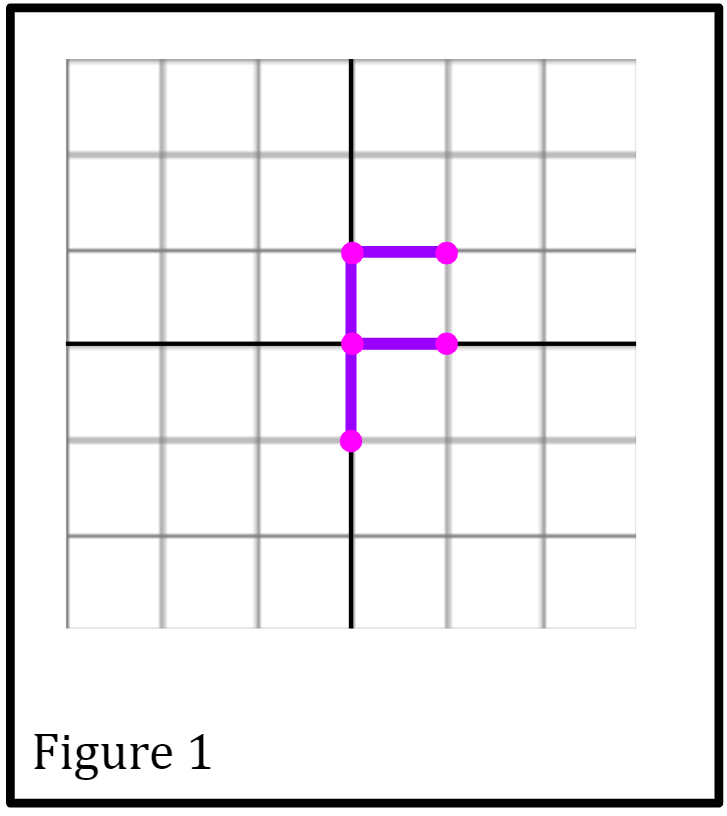
\includegraphics[scale=0.3]{../assets/f0.png}
\end{center}
We assume that the grid lengths are unit lengths. 

\begin{mdframed}[]
    (Example.) Consider the transformation 
    \[A: \cyclic{x, y} \mapsto \cyclic{-y, x}.\]
    Using the ``F''-shape above, this transformation maps it to: 
    \begin{center}
        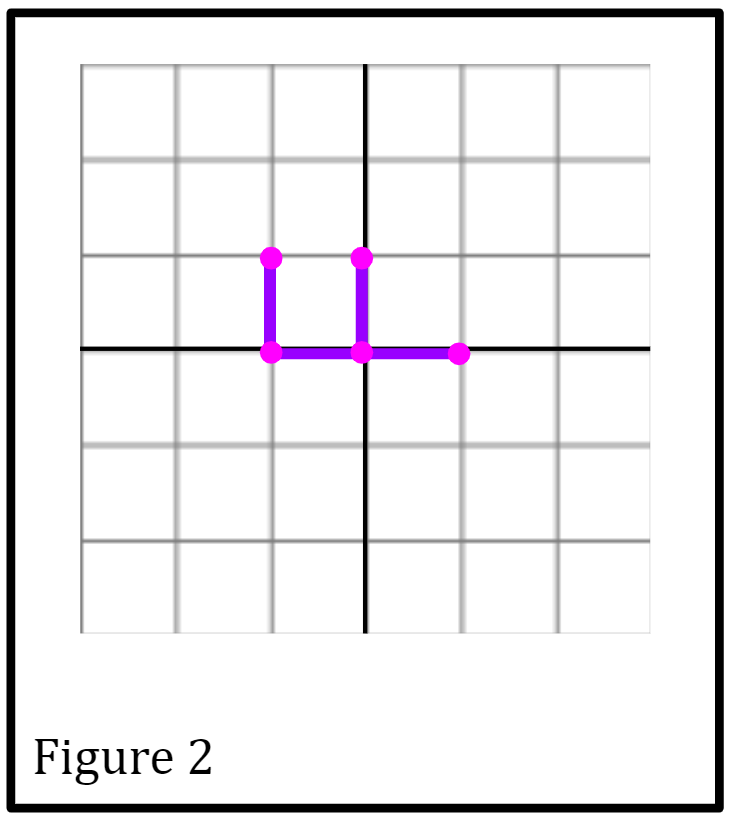
\includegraphics[scale=0.3]{../assets/f1.png}
    \end{center}
\end{mdframed}

\begin{mdframed}[]
    (Example.) Consider the \emph{shearing} transformation
    \[A: \cyclic{x, y} \mapsto \cyclic{x + y, y}.\]
    Using the ``F''-shape above, this transformation maps it to: 
    \begin{center}
        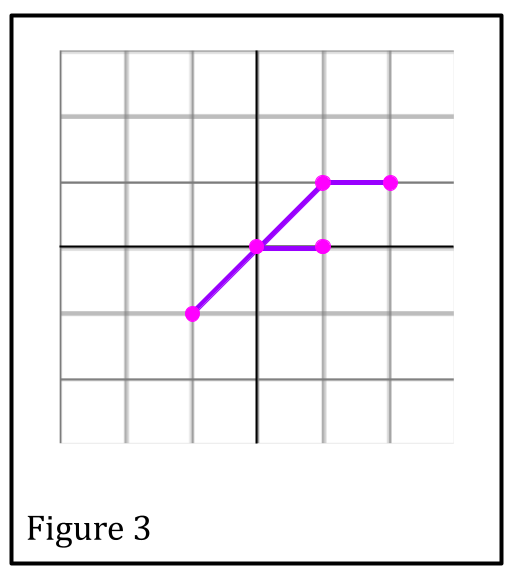
\includegraphics[scale=0.3]{../assets/f2.png}
    \end{center}
\end{mdframed}

\begin{mdframed}[]
    (Example.) Consider the \emph{scaling} transformation\footnote{If $\alpha$ and $\beta$ are scalars that scale the $x$- and $y$-component, respectively, then $S_{\alpha, \beta}(\cyclic{x, y}) = \cyclic{\alpha x, \beta y}$.}
    \[A: \cyclic{x, y} \mapsto \cyclic{2x, \frac{1}{2}y} \qquad S_{\cyclic{2, \frac{1}{2}}}.\]
    Using the ``F''-shape above, this transformation maps it to: 
    \begin{center}
        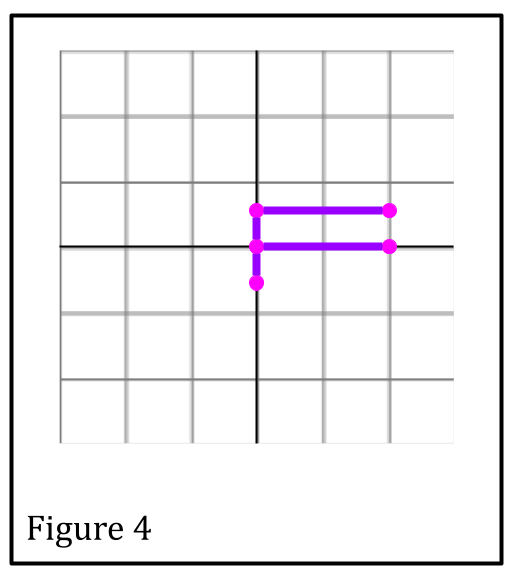
\includegraphics[scale=0.3]{../assets/f3.png}
    \end{center}
\end{mdframed}

\begin{mdframed}[]
    (Example.) Consider the following affine transformation
    \[A(\mathbf{x}) = (T_{\cyclic{2, 1}} \circ R_{90^{\circ}})(\mathbf{x}) = A(\mathbf{x}) = R_{90^{\circ}}(\mathbf{x}) + \cyclic{2, 1}.\]
    The idea is that, for $\cyclic{x_0, x_1} \in \R^2$, we have
    \[A(\cyclic{x_0, x_1}) = \cyclic{-x_1, x_0} + \cyclic{2, 1} = \cyclic{-x_1 + 2, x_0 + 1}.\]
    Using the ``F''-shape above, this transformation maps it to: 
    \begin{center}
        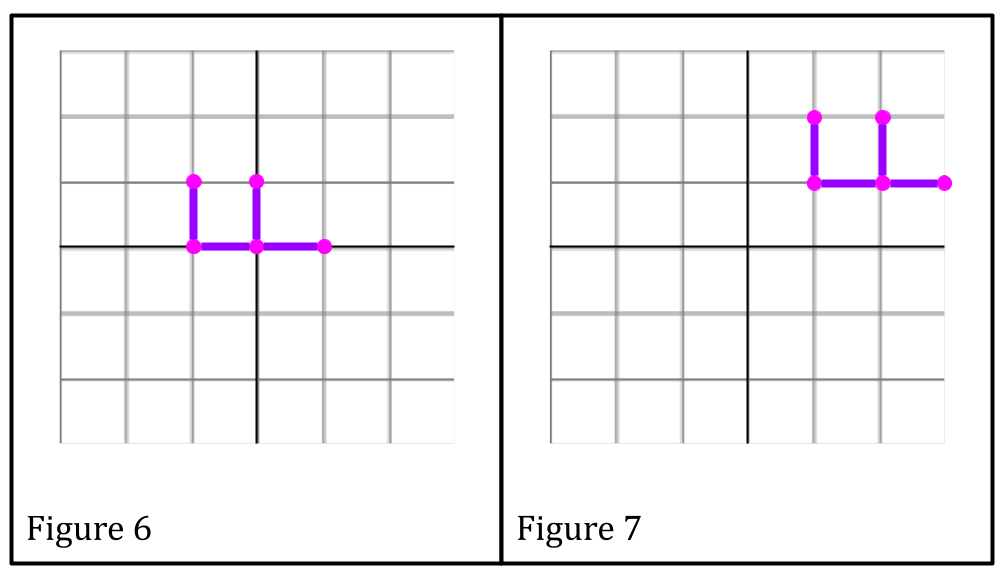
\includegraphics[scale=0.3]{../assets/f5.png}
    \end{center}
    Here, figure (6) shows the rotation by 90 degrees counter-clockwise, while figure (7) shows the translation. 
\end{mdframed}


\subsection{Matrix Representation \& Rotations}
In this section, assume that: 
\begin{itemize}
    \item $\R^2$ is the 2-dimensional vector space.
    \item Points $\mathbf{x}$ and $\mathbf{y}$ are column vectors $\mathbf{x} = \begin{bmatrix}
        x_1 \\ x_2
    \end{bmatrix} = \cyclic{x_1, x_2}$. 
    \item The linear transformation is defined by the mapping $A: \R^2 \mapsto \R^2$. 
    \item The standard basis $\mathbf{i}$ and $\mathbf{j}$ is given by 
    \[\mathbf{i} = \cyclic{1, 0} \qquad \mathbf{j} = \cyclic{0, 1}.\]
    \item Let $\mathbf{u} = A(\mathbf{i})$ and $\mathbf{v} = A(\mathbf{j})$, where 
    \[\mathbf{u} = \cyclic{u_1, u_2} \qquad \mathbf{v} = \cyclic{v_1, v_2}.\]
\end{itemize}

\begin{proposition}
    Let $M = \begin{bmatrix}
        u_1 & v_1 \\ u_2 & v_2
    \end{bmatrix}$. This represents $A$ in that
    \[M\mathbf{x} = A(\mathbf{x}).\]
\end{proposition}

\begin{mdframed}[nobreak=true]
    \begin{proof}
        First, note that
        \[M\mathbf{x} = \begin{bmatrix}
            u_1 & v_1 \\ u_2 & v_2
        \end{bmatrix} \begin{bmatrix}
            x_1 \\ x_2
        \end{bmatrix} = \begin{bmatrix}
            u_1 x_1 + v_1 x_2 \\ 
            u_2 x_1 + v_2 x_2
        \end{bmatrix}.\]
        On the other hand, 
        \begin{equation*}
            \begin{aligned}
                A(\mathbf{x}) &= A(x_1 \mathbf{i} + x_2 \mathbf{j}) \\ 
                    &= A(x_1 \mathbf{i}) + A(x_2 \mathbf{j}) && \text{By linearity.} \\ 
                    &= x_1 A(\mathbf{i}) + x_2 A(\mathbf{j}) && \text{By linearity.} \\ 
                    &= x_1 \mathbf{u} + x_2 \mathbf{v} \\ 
                    &= x_1 \begin{bmatrix}
                        u_1 \\ u_2
                    \end{bmatrix} + x_2 \begin{bmatrix}
                        v_1 \\ v_2
                    \end{bmatrix} \\ 
                    &= \begin{bmatrix}
                        u_1 x_1 + v_1 x_2 \\ 
                        u_2 x_1 + v_2 x_2
                    \end{bmatrix}.
            \end{aligned}
        \end{equation*}
        Thus, we are done. 
    \end{proof}
\end{mdframed}
\textbf{Remark:} The moral of the story is that we look at the action of the transformation on the standard basis vectors, which gives us values $\mathbf{u}$ and $\mathbf{v}$; the columns of the matrix $M$ are equal to the images (the values) of $A$ on the vectors $\mathbf{i}$ and $\mathbf{j}$.

\begin{mdframed}[]
    (Example.) Consider the linear transformation $A$ that takes the ``F''-shape from Figure (1) and transforms it to the following ``F''-shape:
    \begin{center}
        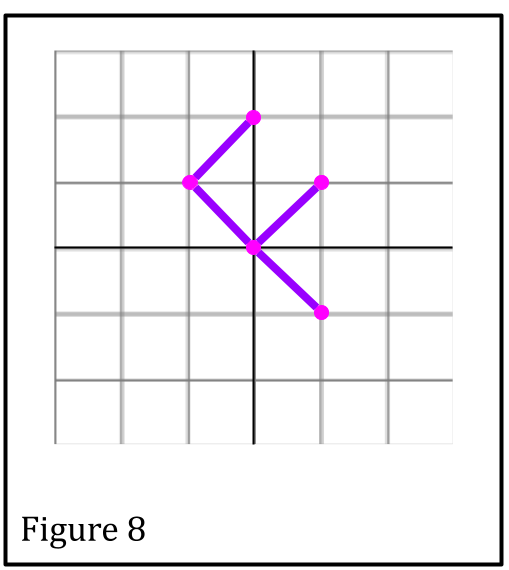
\includegraphics[scale=0.3]{../assets/f6.png}
    \end{center}
    We want to find the matrix representing $A$. To do so, we consider the image of the standard basis vectors $\mathbf{i} = \begin{bmatrix}
        1 \\ 0
    \end{bmatrix}$ and $\mathbf{j} = \begin{bmatrix}
        0 \\ 1
    \end{bmatrix}$. So: 
    \begin{center}
        \begin{tabular}{c|c|c}
            \textbf{Old Point} (Figure 1) & \textbf{Transformed Point, i.e. Image} (Figure 8) & \textbf{Vector Form} \\ 
            \hline 
            $\mathbf{i} = \cyclic{1, 0}$ & $\cyclic{1, 1}$ & $\mathbf{u} = \begin{bmatrix}
                1 \\ 1
            \end{bmatrix}$ \\ 
            $\mathbf{j} = \cyclic{0, 1}$ & $\cyclic{-1, 1}$ & $\mathbf{v} = \begin{bmatrix}
                -1 \\ 1
            \end{bmatrix}$
        \end{tabular}
    \end{center}

    Thus, the matrix representing $A$ is $\begin{bmatrix}
        \mathbf{u} & \mathbf{v}
    \end{bmatrix} = \begin{bmatrix}
        1 & -1 \\ 1 & 1
    \end{bmatrix}$.
\end{mdframed}

\begin{mdframed}[nobreak=true]
    (Example.) Let $R_{\theta}$ be the transformation by rotating counter-clockwise (CCW) around the origin\footnote{Think of it as if you have a pin which is on the origin. Then, you're rotating the figure about the origin, the pin.} by angle $\theta$. We want the matrix representation of $R_{\theta}$. So, we just need to see what $R_{\theta}$ does to the standard basis vectors. 
    \begin{center}
        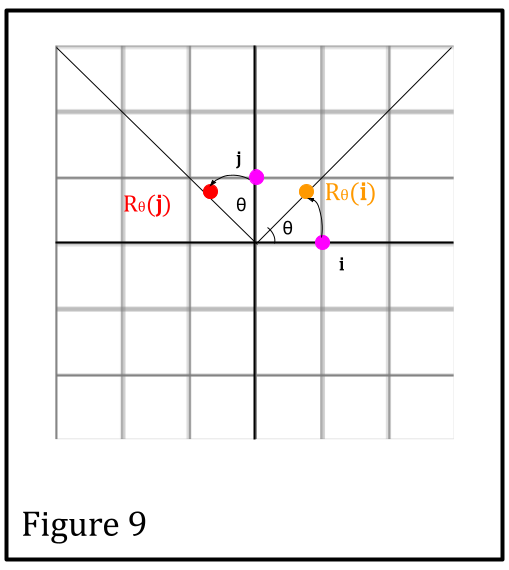
\includegraphics[scale=0.4]{../assets/f7.png}
    \end{center}
    Here, we have 
    \[R_{\theta}(\mathbf{i}) = \cyclic{\cos \theta, \sin \theta} \qquad R_{\theta}(\mathbf{j}) = \cyclic{-\sin \theta, \cos \theta}.\]
    This gives us the matrix 
    \[\begin{bmatrix}
        \cos \theta & -\sin \theta \\ 
        \sin \theta & \cos \theta
    \end{bmatrix}.\]
    What does this mean for representing affine transformations? 
\end{mdframed}

\begin{mdframed}[]
    (Example.) Consider the \emph{affine} transformation $A$ that takes the ``F''-shape from Figure (1) and transforms it to the following ``F''-shape:
    \begin{center}
        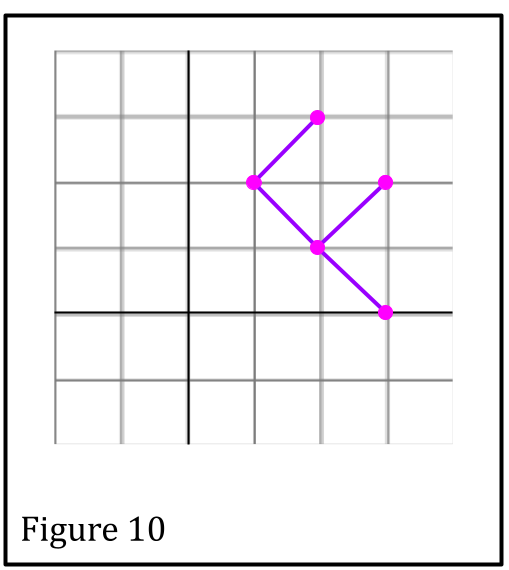
\includegraphics[scale=0.3]{../assets/f8.png}
    \end{center}
    \emph{In the previous examples} under this section, the origin of the transformed ``F''-shape was still on the origin. So, the vector image was always given by $\mathbf{u} = A(\mathbf{i}) - \mathbf{i} = \cyclic{i_0 - 0, i_1 - 0}$ and $\mathbf{v} = A(\mathbf{j}) - \mathbf{j} = \cyclic{j_0 - 0, j_1 - 0}$. This is not the case here. 
    
    \bigskip
    
    We note that the $\mathbf{i}$ vector from the original ``F''-shape (that is, from $\cyclic{0, 0}$ to $\cyclic{1, 0}$) has been mapped to the image $A(\mathbf{i})$ vector (that is, from $\cyclic{2, 1}$ to $\cyclic{3, 2}$). We see that $A(\mathbf{i})$ is thus the vector $\cyclic{3 - 2, 2 - 1} = \cyclic{1, 1}$. Note that we just took the difference of the two components of the points in the image. 

    \bigskip 

    Likewise, the $\mathbf{j}$ vector from the original ``F''-shape (that is, from $\cyclic{0, 0}$ to $\cyclic{0, 1}$) has been mapped to the image $A(\mathbf{j})$ vector (that is, from $\cyclic{2, 1}$ to $\cyclic{1, 2}$). We see that $A(\mathbf{j})$ is thus the vector $\cyclic{1 - 2, 2 - 1} = \cyclic{-1, 1}$. 

    \bigskip 

    We also note that there is a translation of $\cyclic{2, 1}$. Therefore, $A(\mathbf{x})$ is given by
    \[A(\mathbf{x}) = \overbrace{\begin{bmatrix}
        1 & -1 \\ 1 & 1
    \end{bmatrix} \begin{bmatrix}
        x_1 \\ x_2
    \end{bmatrix}}^{\text{Linear part.}} + \underbrace{\begin{bmatrix}
        2 \\ 1
    \end{bmatrix}}_{\text{Translation.}}.\]
\end{mdframed}

\end{document}